% Setup -------------------------------

\documentclass[a4paper]{report}
\usepackage[a4paper, total={6in, 10in}]{geometry}
\setcounter{secnumdepth}{3}
\setcounter{tocdepth}{3}

\usepackage{hyperref}

% Images package
\usepackage{graphicx}
\usepackage{caption}
\usepackage{subcaption}

% Encoding
%--------------------------------------
\usepackage[T1]{fontenc}
\usepackage[utf8]{inputenc}
%--------------------------------------

% Portuguese-specific commands
%--------------------------------------
\usepackage[portuguese]{babel}
%--------------------------------------

% Hyphenation rules
%--------------------------------------
\usepackage{hyphenat}
%--------------------------------------

% Capa do relatório

\title{
	Computação Avançada
	\\ \Large{\textbf{Projeto de Avaliação}}
	\\ -
	\\ Mestrado em Engenharia Informática
	\\ \large{Universidade do Minho}
	\\ Relatório
}
\author{
	\begin{tabular}{ll}
		\textbf{Grupo}
		\\\hline
		PG41081 & José Alberto Martins Boticas
		\\
		PG41090 & João Ribeiro Imperadeiro
		\\
		PG41091 & Nelson José Dias Teixeira
	\end{tabular}
}

\date{\today}

\begin{document}

\begin{titlepage}
    \maketitle
\end{titlepage}

% Resumo

\begin{abstract}
	Este projeto de avaliação relativo à unidade curricular de Computação Avançada consiste, globalmente, em instalar e configurar um \textit{cluster} de \textit{HTCondor} 
	com pelo 3 nós e utilizar o mesmo na resolução de uma tarefa de processamento (compressão de um vídeo, em \textit{mp4}).
\end{abstract}

% Índice

\tableofcontents

% Introdução

\chapter{Introdução} \label{intro}
\large{
	De forma sucinta, neste trabalho prático é pedida a implementação de um \textit{cluster} \textit{HTCondor} para a realização de tarefas de processamento de grandes volumes de 
	dados ou de elevada complexidade. Para além disso, como seria de esperar, é necessário especificar o sistema desenvolvido pelos elementos deste grupo bem como aspetos adicionais associados ao mesmo.
	
	Neste caso em concreto, é pedido algo mais específico, isto é, o desenvolvimento de uma aplicação de \textit{resizing} de vídeo. Através deste caso, é possível mostrar o funcionamento do \textit{cluster} em questão, transformando, por exemplo, um determinado vídeo com resolução \textit{fullHD} (1080p) na resolução \textit{SD} (720p).

	A correta realização desta tarefa passa por reduzir o tempo necessário à conversão do vídeo em causa. Como tal, é possível partir o vídeo original em vários segmentos, fazendo a conversão	de cada um destes e, no fim, juntá-los todos no vídeo de resultado. Seguindo a sugestão do docente desta unidade curricular, foi utilizado o comando \textit{ffmpeg} para auxiliar a	execução deste tipo de tarefa.
}

\chapter{Implementação}

    \section{Instalação e configuração do cluster}
	Antes de iniciarmos o desenvolvimento da solução para a realização da tarefa proposta, foi necessário configurarmos algumas máquinas, parte integrante do nosso cluster. Para isso, recorremos ao serviço DigitalOcean, onde é possível alugar máquinas virtuais. Assim, e dado que no enunciado são pedidas, no mínimo, 3 máquinas (valor este facilmente escalável a outros números de máquinas), alugamos 3 servidores virtuais (com 1 núcleo de processamento e 1GB de memória ram), os quais interligamos recorrendo a ligações provadas fornecidas pelo serviço.
	
	Posto isto, fizemos a configuração inicial das máquinas, utilizando o sistema operativo CentOS, na versão 7, e seguimos os passos de instalação do HTCondor, ferramenta para criação de clusters, tal como indicado pelo docente num ficheiro na Dropbox.
	tendo em conta que num sistema HTCondor há a noção de master e worker, tomámos a decisão de criar: 1 máquina master, que recebe os pedidos dos clientes e trata do processamento e eventual divisão de trabalho pelos workers, devolvendo uma resposta no fim do processamento; 3 máquinas worker, sendo que uma delas é a master, que estão responsáveis por efetuar tarefas pedidas pelo master.
	
	Desta forma, o nosso cluster está configurado e pronto a receber tarefas para executar.
    
    \section{Realização da tarefa}
    Tendo o cluster configurado, o passo seguinte foi o desenvolvimento dos scripts que nos permitem executar a tarefa proposta. Esta tarefa consiste na receção de um vídeo na resolução 1080p de um utilizador pelo master. Por sua vez, o master procede à sua divisão em 3 partes iguais, enviando cada uma delas para cada um dos workers. Estes workers comprimem a sua parte do vídeo para a resolução 720p, tarefa esta que demora uma quantidade significativa de tempo, o que a torna ideal para este tipo de sistema de cluster. De seguida, os workers enviam a sua parte do vídeo, já comprimida, para o master, sendo que este junta todas as partes e devolve o vídeo comprimido ao cliente.
    
    Para atingirmos este objetivo, proposto no enunciado, decidimos desenvolver vários scripts. O primeiro deles é um script DAG, que será submetido com o comando \textit{condor\_submit\_dag} do HTCondor, e especifica a ordem das operações.

	\begin{figure}[h]
		\centering
		\begin{subfigure}{.5\textwidth}
			\centering
			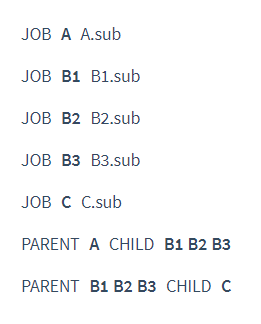
\includegraphics[width=.4\linewidth]{DAG.png}
			\caption{Código da tarefa}
			\label{fig:sub1}
		\end{subfigure}%
		\begin{subfigure}{.5\textwidth}
			\centering
			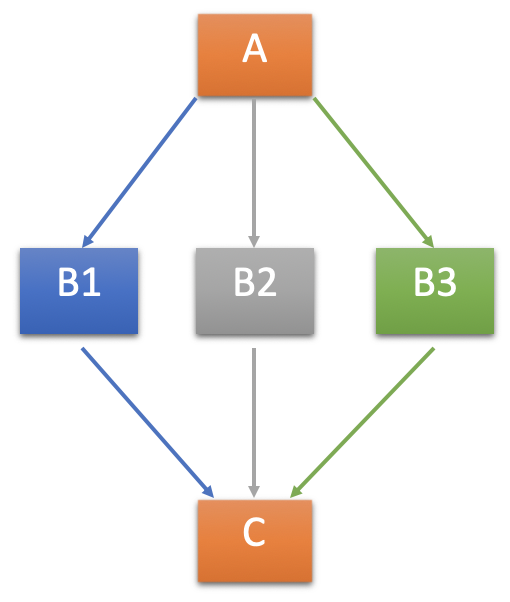
\includegraphics[width=.4\linewidth]{Arquitetura-HTCondor.png}
			\caption{Desenho da tarefa}
			\label{fig:sub2}
		\end{subfigure}
		\caption{Planificação da tarefa}
		\label{fig:dag}
	\end{figure}

	No código acima, juntamente com o respetivo diagrama, podemos ver o nosso script, que indica ao HTCondor a ordem e a dependência das operações a realizar na tarefa. Em primeiro lugar, especificamos o trabalho A, onde o vídeo é divido em 3 partes iguais. De seguida, definimos 3 trabalhos, o B1, B2 e B3, que correspondem ao processo de compressão de cada uma das 3 partes do vídeo. Como especificado no script, estes 3 trabalhos dependem dp trabalho A, pois é necessário as 3 partes existirem antes de os workers as poderem comprimir. Por último, é definido o trabalho C, dependente do B1, B2 e B3, que corresponde ao processo de junção das 3 partes comprimidas num só vídeo.
	
	Passando agora às operações individuais, começamos por apresentar a de dividir o vídeo em 3 partes de igual comprimento.
	
	% Inserir A:sub
	
	Como podemos ver, é utilizada uma das muitas vertentes da ferramenta ffmpeg para dividir o vídeo, sendo que o ficheiro do vídeo (fragmento.mp4) é indicado como sendo o input.
	
	De seguida, temos as 3 operações de compressão das partes do vídeo. Dado que os 3 scripts são semelhantes, apresentaremos apenas um deles.
	
	% Inserir B*.sub
	
	Mais uma vez, é utilizada a ferramenta ffmpeg, recebendo como input a parte correspondente a cada uma das tarefas, dependendo do worker.
	
	Por fim, vem a operação de junção das 3 partes do vídeo. Como o ffmpeg é muito versátil, utilizamos mais uma das suas capacidades, permitindo-nos obter o vídeo pretendido.
	
	% Inseror C.sub
	
	Este script recebe como inputs um ficheiro contendo os caminhos para as diferentes partes do vídeo e as 3 partes do vídeo em si.

\chapter{Conclusão}
\large{
	Para concluir, foi possível, de uma forma muito simples, configurarmos um cluster virtual utilizando o HTCondor, de forma a comprimir um vídeo, tarefa naturalmente muito exigente do ponto de vista computacional, ao dividirmos o trabalho por 3 máquinas diferente, acelerando este processo.
	Assim, foi-nos possível pormos em prática os conhecimentos adquiridos na parte de HTC da Unidade Curricular de Computação Avançada, o que nos permitiu experimentar com máquinas virtuais na cloud e as ferramentas HTCloud/ffmpeg.
	Por fim, consideramos que a nossa resolução foi muito positiva, ao utilizarmos diversas funcionalidades das ferramentas propostas e ainda termos utilizado o ambiente de máquinas virtuais do HTCondor.
}

\chapter{Webgrafia}
    \begin{itemize}
        \item Documentação - \textbf{\textit{ffmpeg}}:
        \par \textit{\url{https://www.ffmpeg.org/ffmpeg.html}}
    \end{itemize}

\appendix
\chapter{Observações}

\end{document}
